% !TeX spellcheck = hu_HU
%----------------------------------------------------------------------------
\chapter{Fejlesztést segítő eszközök}
%----------------------------------------------------------------------------
A fejlesztés során igyekeztem minél több olyan eszközt használni, ami elősegíti a munkát és javítja a kódminőséget és biztonságot.
%----------------------------------------------------------------------------

\section{Continuous Integration}
A Continuous Integration napjainkban már elengedhetetlen része a fejlesztési folyamatoknak.
Rengetek megoldás létezik, azonban én a GitHub Action mellett döntöttem.
Ennek oka, hogy a GitHub–ot használtam a verziókezelt kód tárolására, így kézenfekvő volt ennek a megoldásnak az alkalmazása.

Az alkalmazást 2 külön repository–ban kezeltem, hogy jobban elkülönüljön a frontend és a backend kódja.
Ennek a hátránya az volt, hogy bár ugyanazon nyelvet használja a két repository mégis kétszer kellett implementálnom a GitHub Action–öket.

Az action–ök létrehozását egyszerű szöveges formában tehetjük meg. 
A \lstinline|.github/workflows| mappába létrehozott github \lstinline|.yml| és \lstinline|.yaml| kiterjesztésű fájlok automatikusan kiértékelődnek a GitHub Action által.

\begin{figure}[!ht]
  \centering
  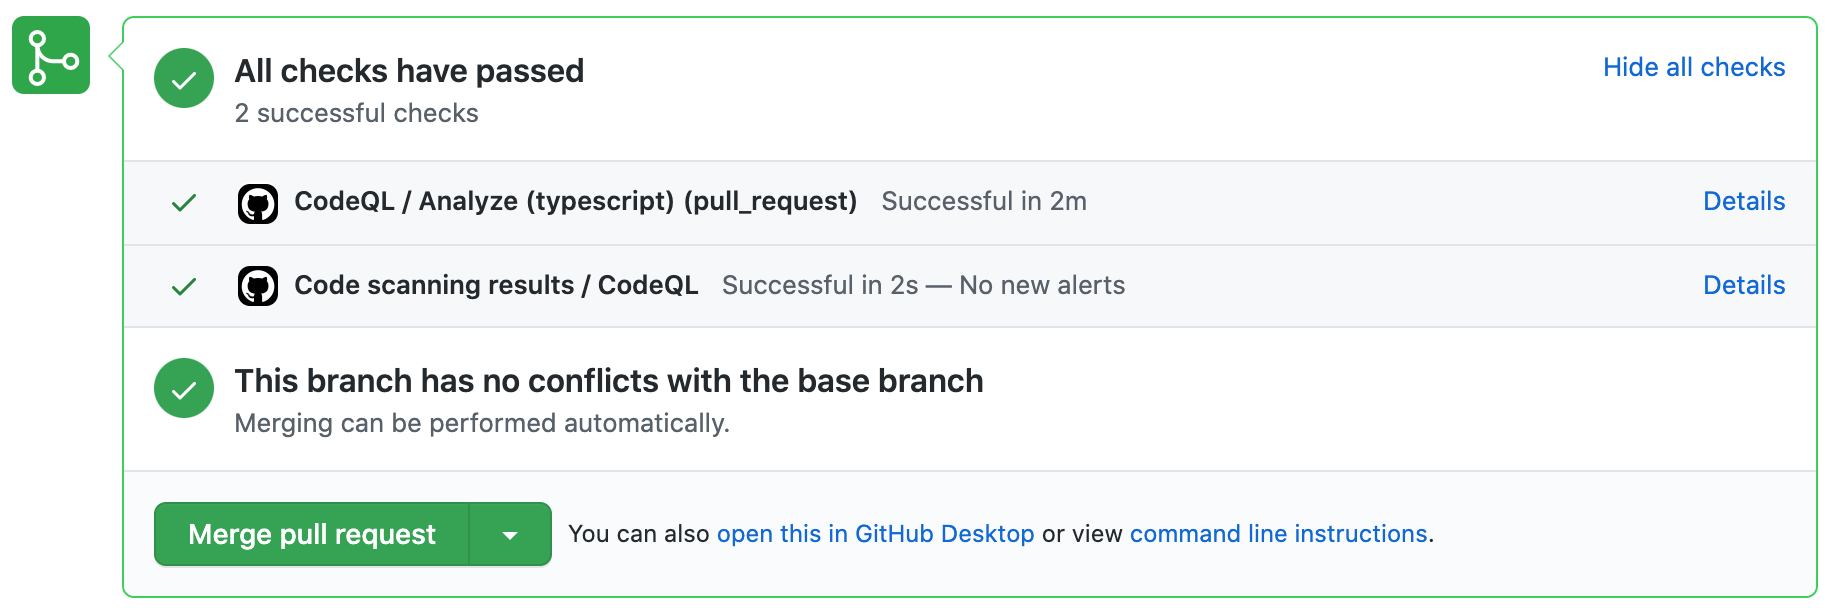
\includegraphics[width=150mm, keepaspectratio]{figures/ci.png}
  \caption{GitHub Action működés közben}
  \label{fig:GitHubAction}
\end{figure}
%----------------------------------------------------------------------------

\subsection{Statikus kódellenőrzés}

\subsubsection{Linter}
A linter egy viszonylag gyors lefutású és kevés erőforrást igénylő action, ezért beállítása szerint bármilyen commit kerül a GitHub repository–ba azonnal lefut és ellenőrzi a kód formázását és jelzi az esetleges hibákat statikus kódellenőrzés segítségével.


%----------------------------------------------------------------------------
\subsubsection{Sercurity check}
A statikus kódellenőrzés egy másik lehetséges felhasználási módja a biztonsági rések keresése, ezt egy a GitHub által ajánlott megoldással valósítottam meg, a CodeQL–lel.
Mivel ez egy több erőforrást igénylő folyamat, ezért a futtatása nem történik meg minden commitnál, csak ha az a főágba történik, vagy ha Pull Request–et nyit valaki, melynek a cél ága a főág.

A képen (\refstruc{fig:securityCheck}) egy a GitHub által észlelt lehetséges sebezhetőség detektálása látható.
A kód analízis során a rendszer észlelte, hogy shell command futtatása történik úgy, hogy annak tartalma környezeti változóból származik.
A figyelmeztetés jelen esetben egy fals riasztás volt, mert a sérülékeny kódrészlet az alkalmazása futása közben nem érhető el, ugyanis a teszt környezet kialakítására szolgál.

\begin{figure}[!ht]
  \centering
  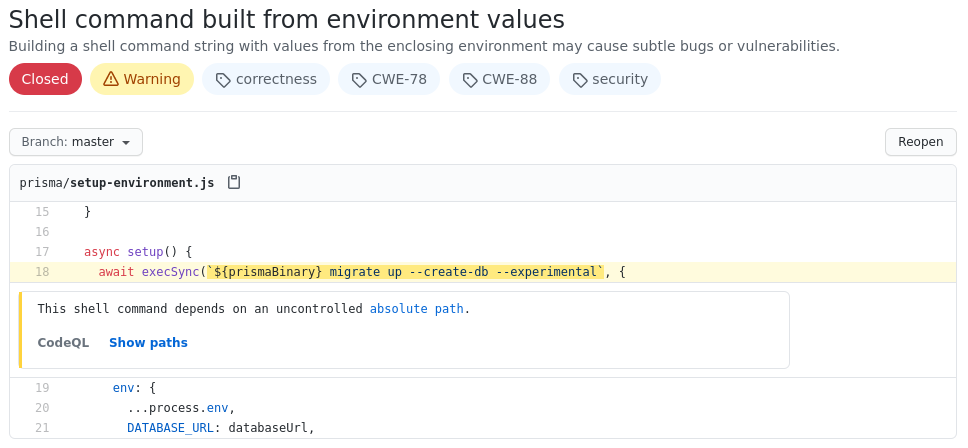
\includegraphics[width=150mm, keepaspectratio]{figures/security.png}
  \caption{Code scanning figyelmeztetés}
  \label{fig:securityCheck}
\end{figure}
%----------------------------------------------------------------------------

\section{Git hook}
Git használata esetén rengeteg eseményhez definiálhatunk úgynevezett hook–okat.
Ezek segítségével bizonyos események után, előtt, vagy közben futtathatunk tetszőleges kódot.
Az alkalmazásomban egy linter–t állítottam be a pre–commit hookra.
Ennek értelmében, új commit elkészítése előtt minden alkalommal lefut a linter így biztosítva a kódminőségét.

\begin{lstlisting}[style=ES6, caption=Pre–commit hook beállításai]    
"husky": {
  "hooks": {
    "pre-commit": "lint-staged"
  }
},
"lint-staged": {
  "*.ts": [
    "eslint --fix"
  ]
}
\end{lstlisting}
  
%----------------------------------------------------------------------------

\section{Continuous Delivery}
A Continuous Integration melett elengedhetetlen része a fejlesztésnek a Continuous Delivery.
A CD\footnote{Continuous Delivery} az alkalmazás folyamatos kitelepítését jelenti, hogy a kód felöltése után szinte azonnal elérhető legyen az szoftverünk legfrissebb változata.

%----------------------------------------------------------------------------

\subsection{Heroku}
A backend alkalmazás üzemeltetésére a Heroku szolgáltatásait vettem igénybe.
Webes felületének és GitHub integrációjának köszönhetően nem igényel komoly szakértelmet az alkalmazás elindítása.
Ingyenes keretek között csak egy ág automatikus kitelepítésére van lehetőség, azonban beállítható az is, hogy megvárja a CI\footnote{Continuous Integration} kimenetelét és csak sikeres futás után kezdje el a telepítést.
Így elkerülhetjük hibás– vagy biztonsági réseket tartalmazó kódok éles környezetbe jutását.

%----------------------------------------------------------------------------

\subsection{Vercel}
A frontend üzemeltetéséhez a Vercel–t használtam. 
A Herokuhoz hasonlóan remek GitHub integrációval és webes felülettel rendelkezik. 
Lehetőségünk nyílik a Pull Request–ekhez egy előnézeti alkalmazás kitelepítésére is, ezzel elősegítve a csapatmunkában egymás munkájának ellenőrzését.
Ilyenkor a Vercel automatikusan hozzáad egy megjegyzést (\refstruc{fig:vercel}) a Pull Requesthez az előnézeti alkalmazás linkjével.

\begin{figure}[!ht]
  \centering
  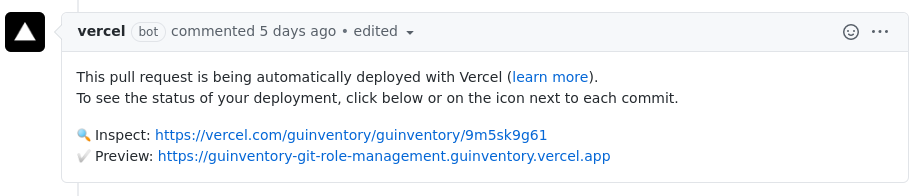
\includegraphics[width=150mm, keepaspectratio]{figures/vercel.png}
  \caption{Vercel megjegyzése Pull Reques–nél}
  \label{fig:vercel}
\end{figure}

%----------------------------------------------------------------------------

